%課題研究レジュメテンプレート ver. 1.2

\documentclass[uplatex]{jsarticle}
\usepackage[top=20mm,bottom=20mm,left=20mm,right=20mm]{geometry}
\usepackage[T1]{fontenc}
\usepackage{txfonts}
\usepackage{wrapfig}
\usepackage[expert,deluxe]{otf}
\usepackage[dvipdfmx,hiresbb]{graphicx}
\usepackage[dvipdfmx]{hyperref}
\usepackage{pxjahyper}
\usepackage{secdot}

\makeatletter
  \renewcommand{\section}{%
    \if@slide\clearpage\fi
    \@startsection{section}{1}{\z@}%
    {\Cvs \@plus.5\Cdp \@minus.2\Cdp}% 前アキ
    {.5\Cvs \@plus.3\Cdp}% 後アキ
    %{\normalfont\Large\headfont\raggedright}}
    {\normalfont\raggedright}}

  \renewcommand{\subsection}{\@startsection{subsection}{2}{\z@}%
    {\Cvs \@plus.5\Cdp \@minus.2\Cdp}% 前アキ
    {.5\Cvs \@plus.3\Cdp}% 後アキ
    %{\normalfont\large\headfont}}
    {\normalfont}}

  \renewcommand{\subsubsection}{\@startsection{subsubsection}{3}{\z@}%
    {\Cvs \@plus.5\Cdp \@minus.2\Cdp}%
    {\z@}%
    %{\normalfont\normalsize\headfont}}
    {\normalfont}}
\makeatother
%ここから上を編集する必要はない.





\title{\vspace{-14mm}Twitterユーザーの興味とリツイート行為の関係分析}
\author{PMコース 矢吹研究室 1442014 岩橋瑠伊}
\date{}%日付を入れる必要はない.
\pagestyle{empty}%ページ番号は振らない.
\begin{document}
\maketitle





\section{研究の背景}
SNSは,コミュニケーションプラットフォームとして私たちにとって大変身近な存在になっている.同時にどのSNSにビジネスの可能性があるかなどの注目も集まっている.
今回は数あるSNSの中からTwitterを選び,Twitterでの広告などのビジネスをより効果的にする手法について考えていく\cite{sns}.

Twitterは2006年7月15日に開設された「ツイート」と称される140文字以内の短文の投稿を共有するウェブ上の情報サービスである.2015年12月時点で,1カ月の間にTwitterにログインしたアクティブユーザー数は3500万人である.世界全体では3億2000万人で約1割が日本国内からのアクセスである\cite{twitter}.

Twitterでは,ツイートをすると自分のフォロワーの見ているタイムラインに自分のツイートが表示される.逆に,自分がフォローしている人がツイートをすると自分のタイムラインにそのツイートが表示される.その他のTwitterの機能にリツイートがある.リツイートとは,元のツイート者のユーザー名のまま自分のフォロワーの見ているタイムラインに転送する機能である.この機能を使うことで自分が興味深い,拡散したいと思ったツイートを自分のフォロワーに伝えられる.

私は自分のタイムラインを読んでいるときに,ユーザーのツイートから判断するにそのユーザーが興味を持っていない内容のツイートに対してリツイートをしている現象を発見した.このことから必ずしもツイートの趣旨とそれをリツイートするユーザーのツイートの趣旨は類似しないと考えた.Twitterで商品の広告を行うとすると,興味を持ったユーザーにリツイートされるのが最も効率が良いと考えられる.つまり,興味を持ったユーザーにリツイートされるようなツイートを作れるようにすれば効率よく広告できるようになるだろう.ツイートを取り巻く環境の変化でリツイートユーザーが変化しているならば,興味を持ったユーザーにリツイートされやすい環境も見つかるのではないかと考えた.

\section{研究の目的}

ツイート内容,公式アカウントであるか非公式アカウントであるか,フォローフォロワー数等の環境変化の下で,ツイートの趣旨とリツイートユーザーのツイートの趣旨の関係性の変化を明らかにする.

\section{プロジェクトマネジメントとの関連}

ツイートの環境によってツイートを伝えたいユーザーの範囲を定められるならば,Twitterで広告を行う企業にとってのステークホルダー・マネジメントになると考えられる.

\section{研究の方法}

最低100リツイート以上されているツイートを集め,そのツイートのリツイートユーザーの中からTwitterAPIを利用して100人(TwitterAPI制限の限界値)のユーザーIDとScreanNameを取り出す.

取得した100人のユーザー全員の最新500ツイート(対象ユーザーの総ツイート数が500に満たない場合は対象ユーザーの全てのツイート)をTwitterAPIで取得する.


取得した100人のユーザーのそれぞれ500ツイートをまとめてMeCabで形態素解析を行い,文章中に含まれる名詞に関してtf-idfで重み付けをするスクリプトを実行する.


これにより抽出された名詞をチェックしていき一つでもリツイートされたツイートの内容と関連する名詞が確認された場合,そのユーザーはリツイートされたツイートの内容と関係があると判断する.


\section{現在の進捗状況}

現在3つのツイートに関して手法の通り分析をし終えており,1つのツイートに関しては分析中である.

分析し終えた3つのツイートは図1のとおりである.図1の左側のツイートから得られた結果を説明していく.企業の公式アカウントが発信するその企業に関連した広告や告知ツイートは100人中80人関係があるという結果となった.図1の真ん中は企業の公式アカウントではないが,一般のユーザーがある企業の情報等を紹介しているツイートの場合100人中62人関係があるという結果となった.

この分析結果より,企業の公式アカウントによる企業の広告や告知はその企業の公式アカウントのフォロワーの種類の時点でユーザーが想定内に定まっていることが分かった.企業の公式アカウントであるという影響力によって,拡散されてもその企業の内容とユーザーが強い関係性を保っていると考えられる.一般のユーザーによる企業の紹介ツイートの例では拡散されていると言ってもあくまで一般のユーザーであり,公式アカウントとしての影響力には程遠い.一般のユーザーは企業の公式アカウントと違い情報の告知や宣伝のためではなく,一般のユーザー視点で興味を持ったユーザーをフォローしていく.その為,拡散されたツイートの内容に相関のないユーザーも多く巻き込んで拡散された結果100人中62人関係性があるという結果になったと考えられる.

図1の右側の結果は100人中6人関係があるという結果となった.

珍しい現象が見られるといったような内容は詳しくその現象について知らなかったとしてもツイートを見た瞬間にリツイートしがち(私がTwitterを利用した際の経験談から)であるということ.そのアカウントが提供する情報が多岐に渡るという点から様々な種類のフォロワーがそのアカウントにいると推測されるため,弱い関係性に繋がったのではないかと考えた.

\begin{figure}[h]
\centering
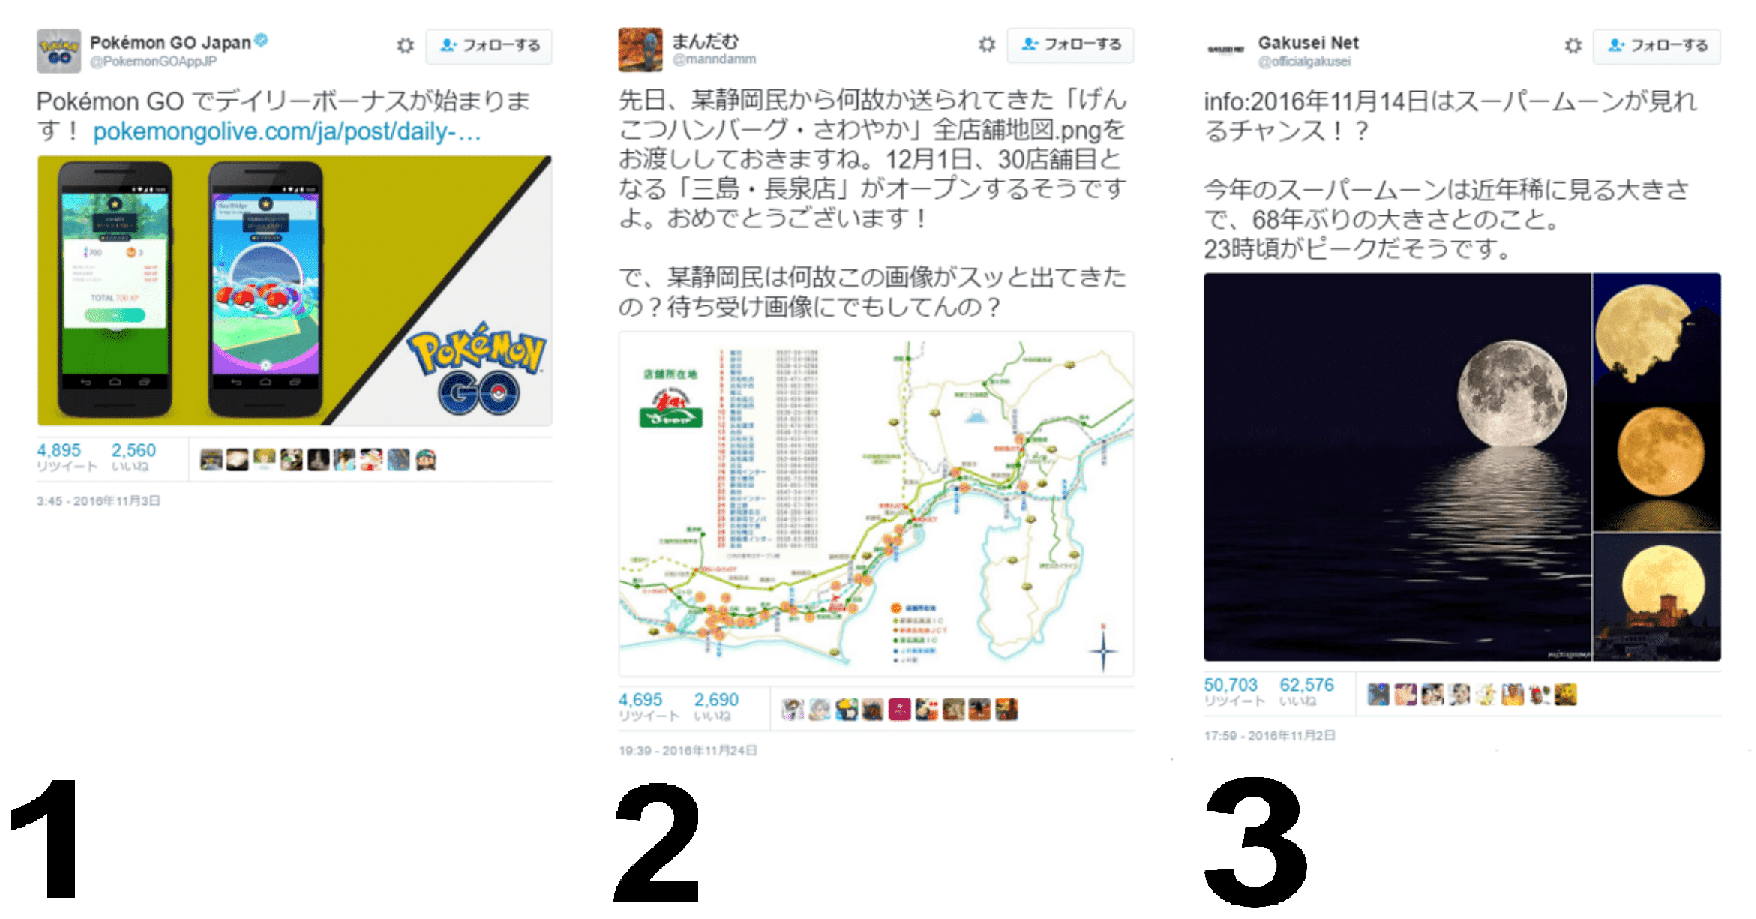
\includegraphics[width=15cm]{g1.pdf}
\caption{分析した3つのツイート}\label{ツイート}
\end{figure}

\section{今後の計画}
\begin{enumerate}
\item まだデータの数が少ないので多くのツイートを分析していくことで仮説検証を行う.
\item 様々な条件のツイートを分析することで新たな仮説を発見する.
\end{enumerate}

\bibliographystyle{junsrt}
\bibliography{biblio}%「biblio.bib」というファイルが必要.

\end{document}
